
\begin{frame}[fragile]{Réseau - côté client}

\begin{lstlisting}
type host_entry = {
	h_addr_list : inet_addr array;
    ...
}
val gethostbyname : string -> host_entry

type socket_domain = PF_UNIX | PF_INET | PF_INET6
type socket_type = 
    | SOCK_STREAM (* TCP *) 
    | SOCK_DGRAM  (* UDP *)
val socket : ?cloexec:bool ->
       socket_domain -> socket_type -> int -> file_descr

type sockaddr = 
    | ADDR_UNIX of string
    | ADDR_INET of inet_addr * int
val connect : file_descr -> sockaddr -> unit
\end{lstlisting}

\end{frame}

\begin{frame}[fragile]{Réseau - côté client - exemple}

\begin{figure}
    \centering
    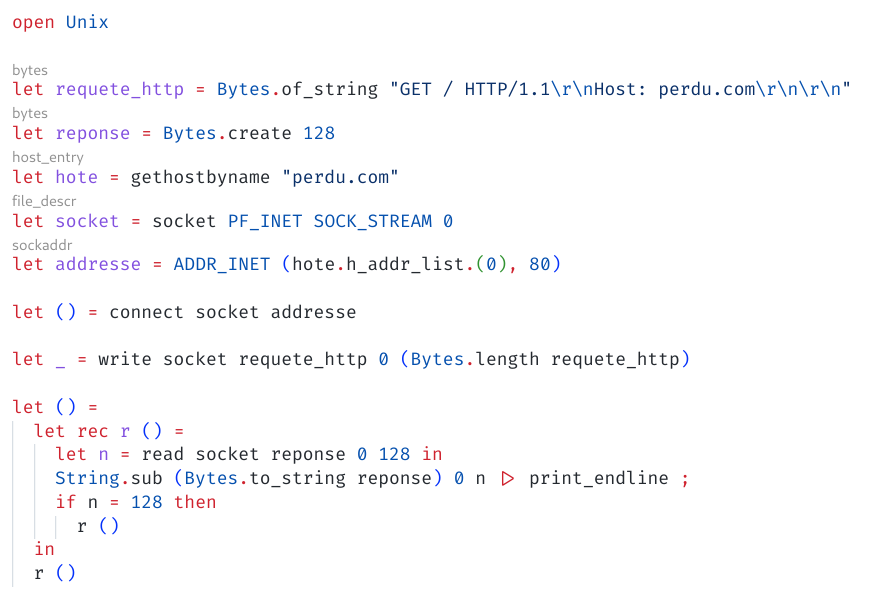
\includegraphics[width=\textwidth]{slides/images/unixsocket.png}
\end{figure}
    
\end{frame}

\begin{frame}[fragile]{Réseau - côté serveur}

\begin{lstlisting}
(* attache la socket à une adresse *)
val bind : file_descr -> sockaddr -> unit
(* met la socket en mode d'écoute *)
val listen : file_descr -> int -> unit
(* accepte une nouvelle connexion *)
val accept : ?cloexec:bool -> file_descr -> file_descr * sockaddr
\end{lstlisting}

\end{frame}

    
\begin{frame}[fragile]{Réseau - côté serveur - exemple}
    
\begin{figure}
    \centering
    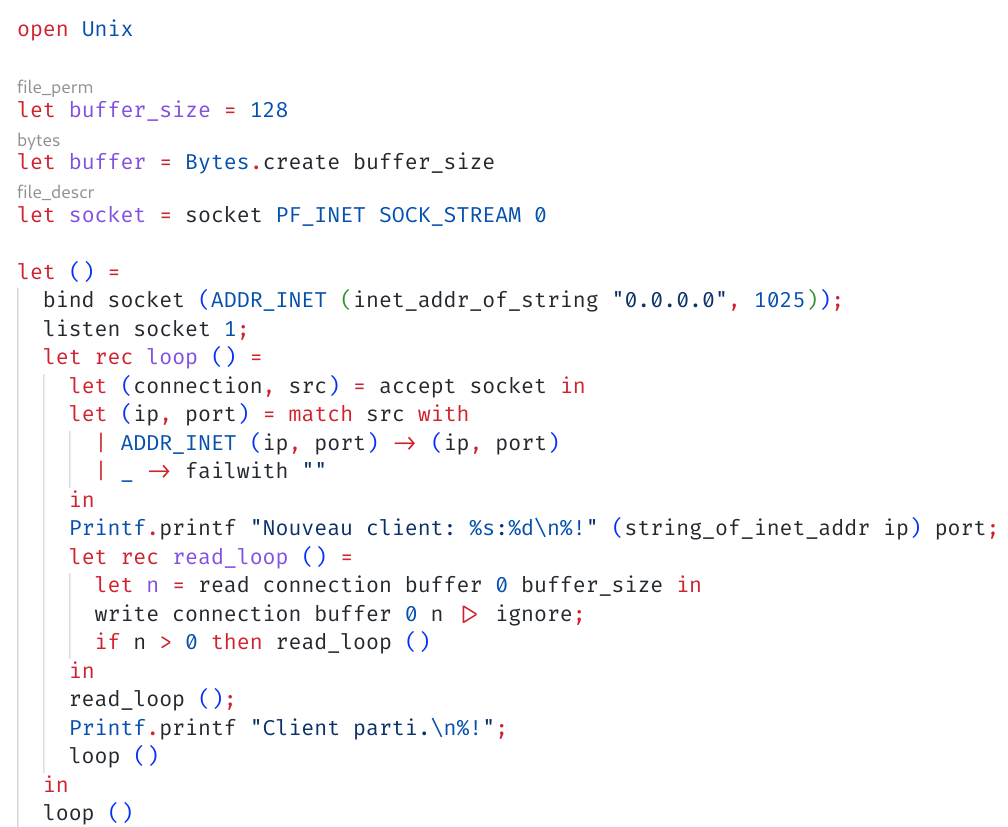
\includegraphics[width=0.9\textwidth]{slides/images/unixsocketserver.png}
\end{figure}

\end{frame}